\documentclass[a4paper]{article}

%% Language and font encodings
\usepackage[british]{babel}

\usepackage{lmodern}
\usepackage[T1]{fontenc}
\usepackage[utf8x]{inputenc}

%% Sets page size and margins
\usepackage[a4paper, margin=1in]{geometry}

%% Useful packages
\usepackage{tikz}
\usetikzlibrary{arrows,shapes,positioning,shadows,trees}

\usepackage{graphicx}
\usepackage[colorinlistoftodos]{todonotes}
\usepackage[colorlinks=true, allcolors=teal]{hyperref}

\usepackage{fontawesome5}

\usepackage[
backend=biber,
style=apa,
sorting=ynt
]{biblatex}
\addbibresource{biblio.bib}

\title{%
\Large Google Summer of Code 2022 \\
\LARGE Differentiable Rendering}

\author{%
\large Contributor: Leonardo D. Mariscal
\href{mailto:l@mariscal.ch}{\faEnvelope} \href{https://github.com/lmariscal}{\faGithub} \href{https://twitter.com/lmariscal_}{\faTwitter} \href{https://www.linkedin.com/in/leomariscal/}{\faLinkedin} \\
\large Mentors: Dhairya Gandhi, Julian Samaroo \\
\large Project Length: 350hr}

\date{}

\tikzset{
every node/.style={draw,text width=3cm,drop shadow},
style1/.style= {rectangle, rounded corners=3pt, thin,align=center,fill=white!60},
style2/.style= {rectangle, rounded corners=3pt, thin,align=center,fill=white!60},
style3/.style= {rectangle,thin,align=left,fill=white!60}
}

\begin{document}
\maketitle

\section*{Abstract}

% Short description of your project. Max 10 sentences. This \textbf{SHOULD
% NOT} be a copy of the project idea text.

% Port the existing project \textit{RayTracer.jl} to make use of the latest Julia version, and update all the underlying libraries. Alongside the port, refactor the automatic differentation extended rules to use the \textit{ChainRules.jl} library, specifically \textit{ChainRulesCore.jl}.\\
% Make use of the already defined components to expand the supported rendering models and implement both \textit{Light Field Networks: Neural Scene Representations
% with Single-Evaluation Rendering} [\cite{NEURIPS2021_a11ce019}], and \textit{Volume Rendering of Neural Implicit Surfaces} [\cite{NEURIPS2021_25e2a30f}].
Port the existing project \textit{RayTracer.jl} to make use of the latest version of Julia, and update all the required libraries. Specially utilise the latest FluxML libraries. Refactor the automatic differentiation (AD) rules to directly target \textit{ChainRulesCore.jl}.

Expand the supported rendering models by using the already defined components, and implement both \textit{Light Field Networks: Neural Scene Representations with Single-Evaluation Rendering} [\cite{NEURIPS2021_a11ce019}], and \textit{Volume Rendering of Neural Implicit Surfaces} [\cite{NEURIPS2021_25e2a30f}].

After finishing the implementation, analyse the performance of all the rendering models inside the project, compare them between themselves, and the original implementations.

Identify both the advantages and disadvantages of changing the output format to \textit{OpenEXR}, and changing the internal data representations to use \textit{Flux3D.jl}.

\section*{Technical Details}

% Long description of the project. \textbf{Must} include all technical
% details of the projects like libraries involved.

% Here it is important to show if you had previous conversations with your
% mentors. You can show relevant pieces of code that you want to change.
% You can link to literature you used during the research.

\section*{Schedule of Deliverables}

% Here should come a list of your milestones. This list is a start based
% on the difference phases of GSoC. Use it as a start. You can/should add
% more details for each phase by breaking it down into weeks or set
% specific targets for each phase. Each target should be split into sub
% task with a time estimate,
% \href{https://en.wikipedia.org/wiki/Work_breakdown_structure}{work
% breakdown structures} are helpful here.

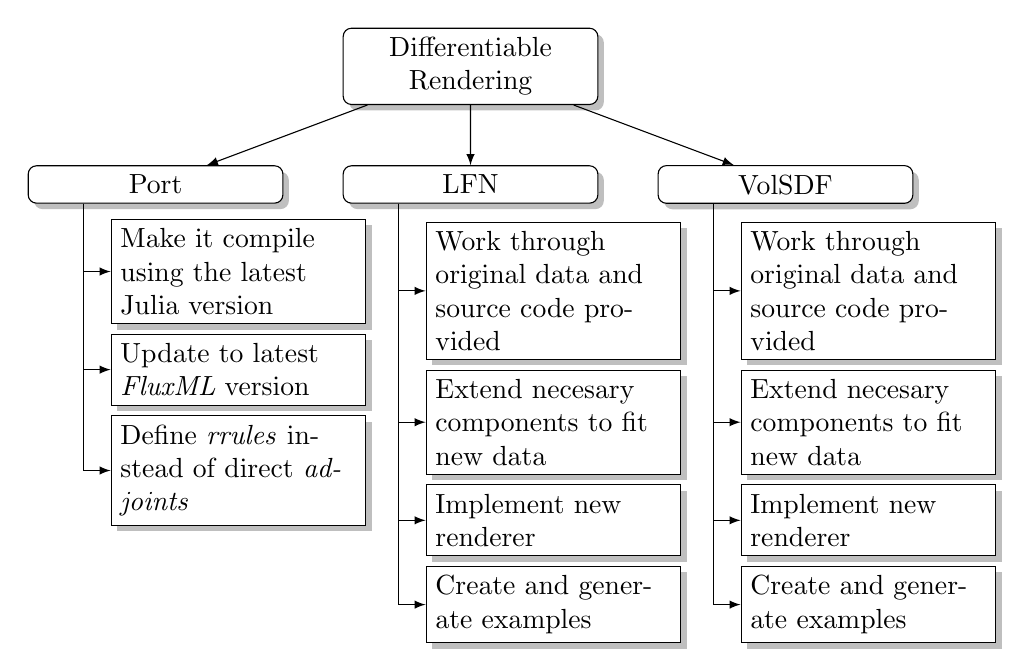
\begin{tikzpicture}[
remember picture,
level 1/.style={sibling distance=40mm},
edge from parent/.style={->,draw},
>=latex]

\node[style1] {Differentiable Rendering}
child {node[style2] (c1) {Port}}
child {node[style2] (c2) {LFN}}
child {node[style2] (c3) {VolSDF}};

\node [style3,below of = c1,xshift=30pt,yshift=-3pt] (c11) {Make it compile using the latest Julia version};
\node [style3,below of = c11,yshift=-7pt] (c12) {Update to latest \textit{FluxML} version};
\node [style3,below of = c12,yshift=-8pt] (c13) {Define \textit{rrules} instead of direct \textit{adjoints}};

\node [style3,below of = c2,xshift=30pt,yshift=-10pt] (c21) {Work through original data and source code provided};
\node [style3,below of = c21,yshift=-19pt] (c22) {Extend necesary components to fit new data};
\node [style3,below of = c22,yshift=-7pt] (c23) {Implement new renderer};
\node [style3,below of = c23,yshift=-2pt] (c24) {Create and generate examples};

\node [style3,below of = c3,xshift=30pt,yshift=-10pt] (c31) {Work through original data and source code provided};
\node [style3,below of = c31,yshift=-19pt] (c32) {Extend necesary components to fit new data};
\node [style3,below of = c32,yshift=-7pt] (c33) {Implement new renderer};
\node [style3,below of = c33,yshift=-2pt] (c34) {Create and generate examples};

\foreach \value in {1,...,3}
  \draw[->] (c1.195) |- (c1\value.west);

\foreach \value in {1,...,4}
  \draw[->] (c2.195) |- (c2\value.west);

\foreach \value in {1,...,4}
  \draw[->] (c3.195) |- (c3\value.west);
\end{tikzpicture}

\subsection*{Community Bonding Period}

% This phase is to get to know the community better. Check that your build
% environment is setup. This time should also be used to discuss your
% project in more detail with the community and in general introduce it.

% \emph{Note:} We require you to write regular blog posts. Now is a good
% time to make sure your blog works and send us the link.

Set up a blog, in order to comply with the blog posts requirement. It will be hosted under\\ \url{https://mariscal.ch/}.

Attend \textit{ML Community + FastAI.jl Dev Call}, previously called \textit{ML and AD Development/Usage Call}s which are hosted every two weeks via zoom, in order to keep up with development and interact with the community.

\pagebreak

\subsection*{Phase 1}

% At the end of Phase 1, \textit{RayTracer.jl} would have already been ported, and the rules written using \textit{ChainRulesCore.jl}. \textit{LFN} implementation should be in development, 
Port \textit{RayTracer.jl} to the latest version of Julia, and update all the libraries used. Update all the \textit{adjoints} to make use of \textit{ChainRulesCore.jl}. Identify if \textit{OpenEXR} would be a better format to set as the output; together with testing if using \textit{Flux3D.jl} to represent the data in some components is adequate. Start with the implementation of \textit{LFN}.

\subsection*{Phase 2}

Finish implementation of both new renderer models, \textit{LFN}, and \textit{VolSDF}. Start by reproducing their results, making use of the provided source-code and their data used, \textit{C++}, and \textit{Python} respectively. Identify how the existing components need to be updated to support all the necessary data. Implement the rendering models, and extend any required \textit{rrules}.

\subsection*{Final Week}

% At this stage you should finish up your project. At this stage you
% should make sure that you have code submitted to your organization. Our
% criteria to mark your project as a success is to submit code before the
% end of GSoC.
Create examples of both render models which would also work as tests of the implementation. Compare all the rendering models, graph performance of all the examples, and if possible, of the original source provided in the papers.

\section*{Development Experience}

% Do you have code on github? Can you show previous contributions to other
% projects? Did you do other code related projects or university courses?
My GitHub profile is \url{https://github.com/lmariscal}. I come with ample experience in real-time rendering, while also keeping up to date with neural scene representation research. Deeply in love with converting data into beautiful 2D images.\\
As for Julia specifically, I have mostly used it for competitive programming challenges, like AdventOfCode. This would be my first big project using this language. Currently using Arch Linux, and feel comfortable using the Julia ecosystem, including the LSP, the package manager, the documentation system, making use of the REPL and its debug features, and in use of the language in general. My main area of focus in the Community phase would be to familiarize myself with the Machine Learning, and Automatic Differentiation libraries the Julia ecosystem has, and that I will be using inside the project. Having made use of both \textit{PyTorch}, and \textit{JAX} in the past, it would mean translating that experience to the Julia ecosystem.

% \section*{Other Experiences}

\section*{Why this project?}

% Why you want to do this project?
My interest in differential rendering started with the publication of \textit{Neural Radiance Fields} [\cite{mildenhall2020nerf}], its ability to generate novel views truly blew my mind. Since then, I have kept up with the literature by attending computer vision, and computer graphics conferences---thankfully they have been virtual these past few years---while also reading journals, and keeping up to date on Arxiv. It took me a while to specifically select these two papers to implement, but they are the ones that most caught my attention, and both of them come with fully open-sourced implementations and the data used.\\
Julia has been one of the languages that was in my radar, but have had no particular project to implement in the language. I feel that this project is perfect to jump into, as it already has a solid base, and it has the promise of demonstrating that Julia is productive and efficient for implementing these kinds of models, while showcasing all of its strengths and its ecosystem. The plan after GSoC is to make use of this project for my Master's thesis, which would itself expand from the work of \textit{LFN} [\cite{NEURIPS2021_a11ce019}].

% \section*{Appendix}

% Extra content

\pagebreak

\printbibliography

\end{document}